\documentclass{article}
\usepackage[utf8]{inputenc}
\usepackage{fancyhdr} % Required for custom headers
%\usepackage{lastpage} % Required to determine the last page for the footer
\usepackage{extramarks} % Required for headers and footers
\usepackage[usenames,dvipsnames]{color} % Required for custom colors
\usepackage{graphicx} % Required to insert images
\usepackage{listings} % Required for insertion of code
\usepackage{courier} % Required for the courier font
\usepackage{lipsum} % Used for inserting dummy 'Lorem ipsum' text into the template
\usepackage{enumerate}
\usepackage{multicol}
\usepackage{caption}
\usepackage{subcaption}
\usepackage{ulem} % underline emph
\usepackage{amsmath} % for \text in mathmode
\usepackage[hypcap]{caption}
\usepackage{diagbox}
\usepackage{slashbox}

% Margins
\topmargin=-0.45in
\evensidemargin=0in
\oddsidemargin=0.5in
\textwidth=5.7in
\textheight=9.0in
\headsep=0.25in

\linespread{1.3} % Line spacing

% Set up the header and footer
\pagestyle{fancy}
\lhead{} % Top left header
\chead{\hmwkClass: \hmwkTitle} % Top center head
\rhead{\firstxmark} % Top right header
\lfoot{\lastxmark} % Bottom left footer
\cfoot{\thepage} % Bottom center footer
%\rfoot{Page\ \thepage\ of\ \protect\pageref{LastPage}} % Bottom right footer
\renewcommand\headrulewidth{0.4pt} % Size of the header rule
\renewcommand\footrulewidth{0.4pt} % Size of the footer rule

\setlength\parindent{0pt} % Removes all indentation from paragraphs

\definecolor{MyDarkGreen}{rgb}{0.0,0.4,0.0} % This is the color used for comments
\lstloadlanguages{C} % Load C syntax for listings, for a list of other languages supported see: ftp://ftp.tex.ac.uk/tex-archive/macros/latex/contrib/listings/listings.pdf
\lstset{language=C, % Use python in this example
        frame=single, % Single frame around code
        basicstyle=\small\ttfamily, % Use small true type font
        keywordstyle=[1]\color{Blue}\bf, % C functions bold and blue
        keywordstyle=[2]\color{Purple}, % C function arguments purple
        keywordstyle=[3]\color{Blue}, % Custom functions \underbar underlined and blue
        identifierstyle=, % Nothing special about identifiers                                         
        commentstyle=\usefont{T1}{pcr}{m}{sl}\color{MyDarkGreen}\small, % Comments small dark green courier font
        stringstyle=\color{Purple}, % Strings are purple
        showstringspaces=false, % Don't put marks in string spaces
        tabsize=4, % 5 spaces per tab
        %
        % Put standard Python functions not included in the default language here
        morekeywords={rand},
        %
        % Put Python function parameters here
        morekeywords=[2]{on, off, interp},
        %
        % Put user defined functions here
        morekeywords=[3]{glutCreateWindow,p},
       	%
        morecomment=[l][\color{Blue}]{...}, % Line continuation (...) like blue comment
        numbers=none, % can use none % Line numbers on left
        firstnumber=1, % Line numbers start with line 1
        numberstyle=\tiny\color{Blue}, % Line numbers are blue and small
        stepnumber=1 % Line numbers go in steps of 5
}
% \usepackage{graphicx}
\newcommand{\indep}{\rotatebox[origin=c]{90}{$\models$}}

% Creates a new command to include a perl script, the first parameter is the filename of the script (without .pl), the second parameter is the caption
\newcommand{\code}[1]{
\begin{itemize}
\item[]\lstinputlisting[label=#1]{#1.c}
%\item[]\lstinputlisting[caption=#2,label=#1]{#1.c}
\end{itemize}
}

%----------------------------------------------------------------------------------------
%	DOCUMENT STRUCTURE COMMANDS
%	Skip this unless you know what you're doing
%----------------------------------------------------------------------------------------

\setcounter{secnumdepth}{0} % Removes default section numbers

\newcommand{\homeworkProblemName}{}
\newenvironment{homeworkProblem}[1]{ % Makes a new environment called homeworkProblem which takes 1 argument (custom name) but the default is "Problem #"
    \renewcommand{\homeworkProblemName}{#1} % Assign \homeworkProblemName the name of the problem
    \section{\homeworkProblemName} % Make a section in the document with the custom problem count
}

\newcommand{\problemAnswer}[1]{ % Defines the problem answer command with the content as the only argument
    \noindent\framebox[\columnwidth][c]{\begin{minipage}{0.98\columnwidth}#1\end{minipage}} % Makes the box around the problem answer and puts the content inside
}

\newcommand{\homeworkSectionName}{}
\newenvironment{homeworkSection}[1]{ % New environment for sections within homework problems, takes 1 argument - the name of the section
    \renewcommand{\homeworkSectionName}{#1} % Assign \homeworkSectionName to the name of the section from the environment argument
    \subsection{\homeworkSectionName} % Make a subsection with the custom name of the subsection
}

%----------------------------------------------------------------------------------------
%	NAME AND CLASS SECTION
%----------------------------------------------------------------------------------------

\newcommand{\hmwkTitle}{Project 2\\ Parallalized 2D Poisson Solver} % Assignment title
\newcommand{\hmwkDueDate}{\date{April 19, 2017}} % Due date
\newcommand{\hmwkClass}{TDT4280} % Course/class
\newcommand{\hmwkAuthorName}{Neshat\ Naderi}  % Your name


%----------------------------------------------------------------------------------------
%	TITLE PAGE
%----------------------------------------------------------------------------------------

\title{
\vspace{2in}
\textmd{\textbf{\hmwkClass:\ \hmwkTitle}}\\
\normalsize\vspace{0.1in}\normalsize{\hmwkDueDate}
\vspace{0.1in}\large{\text{Introduction to Supercomputing}}
\vspace{3in}
}

\author{\textbf{\hmwkAuthorName}}
\date{} % Insert date here if you want it to appear below your name

%----------------------------------------------------------------------------------------
\begin{document}
\maketitle

% \setcounter{tocdepth}{1} % Uncomment this line if you don't want subsections listed in the ToC

% \newpage
% \tableofcontents
%\newpage

%----------------------------------------------------------------------------------------
%	PROBLEM 1
%----------------------------------------------------------------------------------------

% To have just one problem per page, simply put a \clearpage after each problem
\newpage
\begin{homeworkProblem}{Introduction}
\subsection{Poisson Problem}

The two dimensional poisson problem is defined as:
$$ -\nabla^2 u = f \quad\quad in \quad \Omega = (0, 1) \times (0, 1). $$
$$u = 0 \quad\quad \quad \quad on \quad \delta\Omega. $$

Where $f$ is the right hand side function, $u$ is the solution and $\Omega$ is the domain.\\
The solution is achieved by descretizing the problem in finite difference grid with $n+1$ points in each spatial direction, where the grid size is $h=\frac{1}{n}$ .

The 5-point stencil method is applied in descretizing the Laplace operator($\Omega$). \\
Diagonalization and  Discrete Sine Transform(DST) methods are choosen to solve the poisson problem. The diagonalization is applied first and then DST. By applying the DST method $O(n^2logn)$ upperbound of floating points operations is gained. 


\end{homeworkProblem}

\begin{homeworkProblem}{The Parallel Poisson Solver}
The goal of this project is implementing a parallalized 2D-poisson solver. 
The first step is parallalizing the given source code by MPI and OpenMP. Then the results of elapsed time is analysed and compared with different problem sizes. This report describes the methodology of the poisson solver and its performance efficiency. The goal is to partition the given square matrix of data into vectors and distribute those matrix segements to processes. So that the processes operates in parallel. 
A serial implementation of the poisson solver is handed out and the task is to implement a parallel version of that solver.
The multiprocessing and multithreading strategy is described in more details in this section.

\subsection{Parallel program using MPI and OpenMP}

Modifications in the serial code is started by partitioning a square matrix$(M \times M)$ into vectors and distributing $\frac{M}{P}$ vectors to each process. $P$ is the number of processes.
The syncronization and communication between processes is provided by the message passing interface(MPI). MPI library is imported by including header file \texttt{mpi.h}.\\
In the next step the MPI environment is initialized by a given number of processes (\texttt{nproc}).
OpenMP is a shared memory multiprocessing API that is used together with MPI. To apply multithreading with OpenMP, the parallel regions(loops) are marked with \texttt{\#pragma} \texttt{omp} \texttt{parallel} \texttt{for}. So that loop iterations are splitted up among threads and so the threads are run paralleled.
\newpage
\subsection{Load balancing}
In the case, the number of rows in the matrix is not divisible by the number of processes, the work per process should be balanced. In this situation, some processes is given $\frac{M}{p}$ vectors.
Listing \ref{lst:load} shows that the leftover vectors $M \mod p$ are distributed to the last processes. So that they own $\frac{M}{p} + 1$ number of vectors each. 

\begin{lstlisting}[language=C, caption=Load balancing, label=lst:load]
    // load balancing, partition the matrix in vectors
    for (size_t i = 0; i < nproc; i++) {
        local_columns[i] = columns;
        // Distribute the remaining columns to last processes
        if ( rest_columns && i >= last_process_index_start ) {
            local_columns[i] = local_columns[i] + 1;
            rest_columns-- ;
        }
        col_displacements[i] = displacement;
        displacement += local_columns[i];
    }

    for (size_t i = 0; i < nproc; i++) {
        counts[i] = local_columns[i] * local_columns[rank];
        displs[i] = chunk_size;
        chunk_size += counts[i];
    }

    if ( rank >= last_process_index_start && m % nproc ) {
        columns++ ;
    }
\end{lstlisting}
\pagebreak
\subsection{Parallel Implementation of Transform Operation}
In order to use a distributed memory programming model, the transpose function involves \texttt{all-to-all} communication. 
The transpose operation is parallalized in the source code and is called \texttt{parallel\_transpose}. 
In this parallalized version, transpose operation is started by packing the data into sendbuffer. 
The all-to-all communication during transpose operation is done by  \texttt{MPI\_Alltoallv}. This function takes care of all communication. Each process distributed a segement operates on the part assigned to that process. Then the receiving data from each process is stored in recievebuffer. In the end, the recievebuffer is unpacked and the data is placed into the matrix. After the last step the given matrix is transposed. \\
The source code is shown in Listing \ref{lst:transpose}.
\begin{lstlisting}[caption={Parallalized Transpose Operation},label={lst:transpose}]
void parallel_transpose(int rank, int nproc, int m, 
                        double *bt, double *b, 
                        double *sendbuf, double *recvbuf, 
                        int *counts, int *displs, 
                        size_t *local_columns, size_t *col_displacements)
{
    #pragma omp parallel for schedule(static)
    for (size_t p = 0; p < nproc; p++) {
        for (size_t col = 0; col < local_columns[rank]; col++) {
            size_t r_index = col * m + col_displacements[p];
            size_t s_index = displs[p] + col * local_columns[p];

        // copy blocks of matrix into the send buffer
        memcpy( sendbuf + s_index, b + r_index, local_columns[p] * 
                sizeof(double) );
        }
    }
    MPI_Alltoallv( sendbuf, counts, displs, MPI_DOUBLE, recvbuf, 
                    counts, displs, MPI_DOUBLE, MPI_COMM_WORLD );

    #pragma omp parallel for schedule(static)
    for (size_t p = 0; p < nproc; p++) {
        for (size_t col = 0; col < local_columns[rank]; col++) {
            for (size_t c = 0; c < local_columns[p]; c++) {
                size_t r_index = c*local_columns[rank] + displs[p] + col;
                size_t s_index = m * col + col_displacements[p] + c;
                bt[s_index] = recvbuf[r_index];
            }
        }
    }
}
\end{lstlisting}
\end{homeworkProblem}

\begin{homeworkProblem}{Performance Analysis}
\begin{table}
\centering
\begin{tabular}{c|c|c|c|c|c|c}
         \textbf{n}  &   \textbf{p}      & \textbf{t}     &  $\tau\ (s)$ &    \textbf{$u$} & \textbf{$S_p$}& \textbf{$\eta _p$} \\ \hline \hline
512&    1&  1&  4.742250e-01&   6.249888e-02&   -&  -    \\
512&    4&  12& 1.085990e-01&   6.249735e-02&   4.366753e+00&   1.091688e+00 \\
512&    8&  4&  2.005280e-01&   6.249735e-02&   2.364882e+00&   2.956102e-01 \\
512&    16& 8&  7.256050e-01&   6.249888e-02&   6.535581e-01&   4.084738e-02 \\
512&    36& 18& 5.074341e+00&   6.249888e-02&   9.345549e-02&   2.595986e-03 \\ \hline
1024&   1&  1&  1.911259e+00&   6.249972e-02&   -&  -    \\
1024&   2&  8&  2.153310e-01&   6.249800e-02&   8.875912e+00&   4.437956e+00 \\
1024&   4&  16& 2.678350e-01&   6.249781e-02&   7.135957e+00&   1.783989e+00 \\
1024&   16& 8&  7.882380e-01&   6.249972e-02&   2.424723e+00&   1.515452e-01 \\
1024&   36& 18& 4.950787e+00&   6.249972e-02&   3.860516e-01&   1.072365e-02 \\ \hline
2048&   1&  1&  8.084189e+00&   6.249993e-02&   -&  -    \\
2048&   2&  36& 7.216190e-01&   6.249981e-02&   1.120285e+01&   5.601425e+00 \\
2048&   3&  16& 1.002780e+00&   6.249991e-02&   8.061777e+00&   2.687259e+00 \\
2048&   16& 4&  1.145253e+00&   6.249993e-02&   7.058867e+00&   4.411792e-01 \\
2048&   4&  2&  1.347390e+00&   6.249993e-02&   5.999888e+00&   1.499972e+00 \\
2048&   36& 18& 7.040044e+00&   6.249993e-02&   1.148315e+00&   3.189764e-02 \\ \hline
4096&   1&  1&  3.439144e+01&   6.249998e-02&   -&  -     \\
4096&   4&  16& 2.649360e+00&   6.249995e-02&   1.298104e+01&   3.245259e+00 \\
4096&   12& 36& 2.726301e+00&   6.249998e-02&   1.261469e+01&   1.051224e+00 \\
4096&   18& 8&  3.152753e+00&   6.249998e-02&   1.090838e+01&   6.060213e-01 \\
4096&   2&  3&  6.361214e+00&   6.249994e-02&   5.406427e+00&   2.703214e+00 \\
4096&   36& 18& 9.399781e+00&   6.249998e-02&   3.658749e+00&   1.016319e-01 \\ \hline
8192&   1&  1&  1.457998e+02&   6.250000e-02&   -&  -     \\
8192&   8&  12& 9.800463e+00&   6.249999e-02&   1.487683e+01&   1.859604e+00 \\
8192&   8&  16& 9.939969e+00&   6.249999e-02&   1.466804e+01&   1.833504e+00 \\
8192&   12& 36& 1.009025e+01&   6.249997e-02&   1.444958e+01&   1.204131e+00 \\
8192&   36& 4&  1.565453e+01&   6.250000e-02&   9.313585e+00&   2.587107e-01 \\
8192&   36& 18& 1.711667e+01&   6.249999e-02&   8.518000e+00&   2.366111e-01 \\
8192&   4&  2&  2.051611e+01&   6.250000e-02&   7.106603e+00&   1.776651e+00 \\
8192&   4&  1&  3.711160e+01&   6.250000e-02&   3.928686e+00&   9.821716e-01 \\ \hline
16384&  1&  1&  6.174798e+02&   6.250000e-02&   -&  -     \\
16384&  8&  12& 4.076668e+01&   6.250000e-02&   1.514668e+01&   1.893335e+00 \\
16384&  16& 6&  4.088034e+01&   6.250000e-02&   1.510457e+01&   9.440354e-01 \\
16384&  8&  16& 4.126072e+01&   6.250000e-02&   1.496532e+01&   1.870665e+00 \\
16384&  6&  36& 4.144498e+01&   6.249999e-02&   1.489879e+01&   2.483131e+00 \\
16384&  12& 2&  4.310132e+01&   6.250000e-02&   1.432624e+01&   1.193853e+00 \\
16384&  36& 4&  4.914745e+01&   6.250000e-02&   1.256382e+01&   3.489950e-01 \\
16384&  4&  4&  5.177619e+01&   6.250000e-02&   1.192594e+01&   2.981485e+00 \\
16384&  2&  3&  1.125774e+02&   6.250000e-02&   5.484935e+00&   2.742467e+00 
\end{tabular}
\caption{Timing results of parallel program on $Lille$ supercomputer with $n=2^k$, $p$ processes and $t$ threads. $f(x,y) = 2(y - y^2 + x - x^2)$ and  $1\leq p \leq36$.}
\label{table:timing}
\end{table}

% \subsection{Timing Results }
The parallel program is compiled and run on Lille supercomputer. Different combinations of $n=2^k$, $P$ and $t$ are tested. The range for process values are $1 \leq P \leq 36$. In Table \ref{table:timing} some timing results are compared. Remaining test results are attached to the source code as TXT and CSV files which contain timings for executed program with cluster nodes of 1 and 2.  Where $n$ is the problem size, $p$ is the number of processes, $t$ is the number of threads, $\tau$ is the elapsed time, $S_p$ is the speedup and $\eta _p$ is the parallel efficiency achieved by the program.
\end{homeworkProblem}

\clearpage
\begin{homeworkProblem}{Hybrid Model}
The test results in Figure \ref{fig:hyb_vs} show decreasing amount of elapsing time for $n=16384$ and comparison of a pure distributed memory program and a hybrid program. When the number of processes are high, both models result in similar wall times. The hybrid model works better than the pure distributed model for most of process size selections. It shows more stability for various $p$ size.\\
A good timing result is achieved by $P\in \{6, 12, 18\}$ and $t\in \{6, 3, 2\}$ for hybrid model documented in Table \ref{table:hybrid_vs}. In those three cases the job is well distributed and the program performs faster. So the program performs better when the number of processes are more than a single process. But too high process size shows poor performance also. As it is shown in Figure \ref{fig:hyb_vs} the curve tends to increase for very high $p$. 

\begin{figure}[h!]
\centering
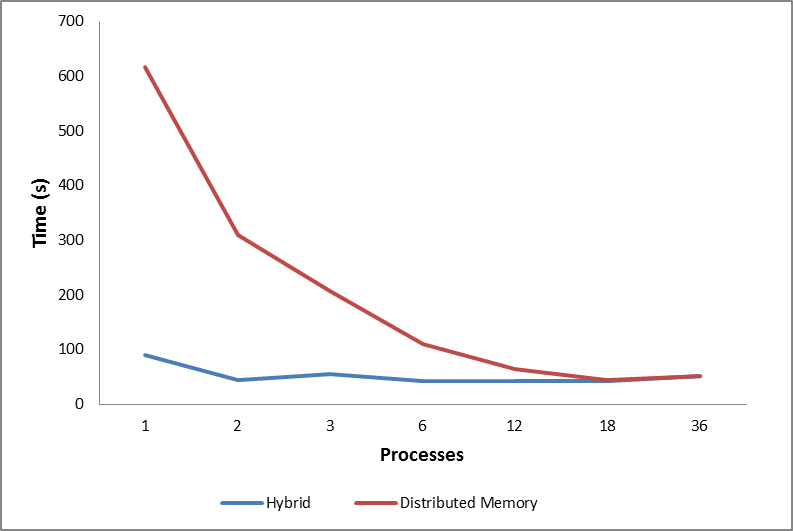
\includegraphics[width=.7\linewidth]{figures/hybridvs16384}
\caption{Hybrid model is compared to distributed memory parallel program for $n = 2^{14} = 16384$ }
\label{fig:hyb_vs}
\end{figure}

\begin{table}[h!]
\centering
\begin{tabular}{c||c|c||c|c}
% \hline
% &\multicolumn{4}{c}{$\tau(s)$ } \\ \hline 
$p$ & $t$ &  Hybrid,  $\tau$ &  $t$ &  Distributed, $\tau$ \\ \hline
1 & 36 & 8.927343e+01 &  1 &6.174798e+02 \\
2 & 18 & 4.441231e+01 &  1 &3.089000e+02 \\
3 & 12 & 5.583350e+01 &  1 &2.073900e+02 \\
6 & 6  & 4.175794e+01 &  1 &1.102293e+02 \\
12 &3 &  4.173763e+01 &  1 &6.365200e+01 \\
18 &2 &  4.183185e+01 &  1 &4.476399e+01 \\
36 &1 &  5.142002e+01 &  1 &5.142002e+01
\end{tabular}
\caption{Hybrid model is compared to distributed memory parallel program with only one thread. For hybrid model $p.t = 36$.}
\label{table:hybrid_vs}
\end{table}

\clearpage
Figure \ref{fig:hyb_n} illustrates how the high process size affect the timing results for three different problem size $n$. The curve's increment tendency is because of the processes' communication overhead. All benchmark results in Table \ref{table:hyb_n} are tested on 2 nodes. \\

\begin{figure}[h!]
\centering
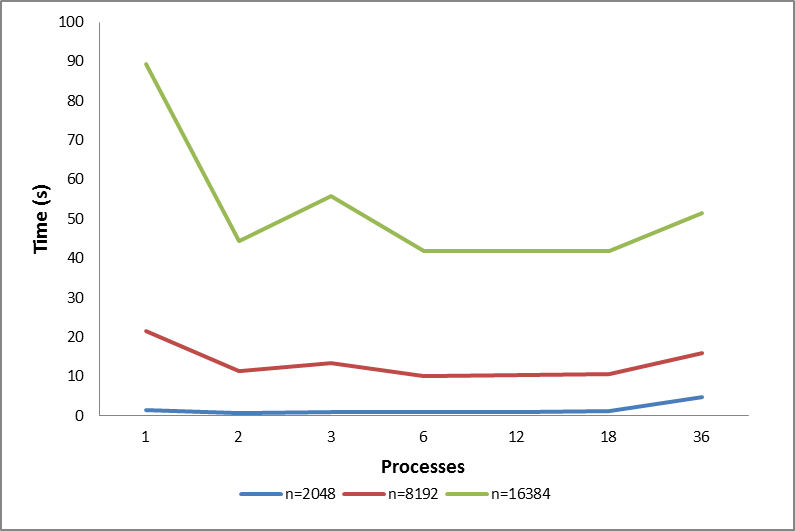
\includegraphics[width=.7\linewidth]{figures/nComparison}
\caption{Decreasing of elapsing time in hybrid model.}
\label{fig:hyb_n}
\end{figure}

\begin{table}[h!]
\centering
\begin{tabular}{c|c|c|c|c}
\hline
\multicolumn{2}{c}{} & \multicolumn{3}{c}{$\tau \ ($\textbf{n}$)$} \\ \hline \hline
\textbf{p}&   \textbf{t}&  2048& 8192 & 16384  \\ \hline
%     % nComp hybrid
1 & 36 &    1.375820e+00 &  2.159030e+01 &  8.927343e+01 \\
2 & 18 &    7.417560e-01 &  1.123698e+01 &  4.441231e+01 \\
3 & 12 &    1.034756e+00 &  1.350203e+01 &  5.583350e+01 \\
6 & 6 & 8.255120e-01 &  1.013905e+01 &  4.175794e+01 \\
12 &    3 & 9.261280e-01 &  1.024582e+01 &  4.173763e+01 \\
18 &    2 & 1.100374e+00 &  1.054620e+01 &  4.183185e+01 \\
36 &    1 & 4.865029e+00 &  1.600261e+01 &  5.142002e+01 \\ \hline
\end{tabular}
\caption{Hybrid model's timing results for different $n$ and $p.t =36$.}
\label{table:hyb_n}
\end{table}

In order to illustrate how thread size for each process can influence the performance, a comparison benchmark is done for various thread numbers. Figure \ref{fig:hyb_th} shows timing differences for $n = 16384$ and that a single thread shows poor performance compared to multiple threads.


\begin{figure}[h!]
\centering
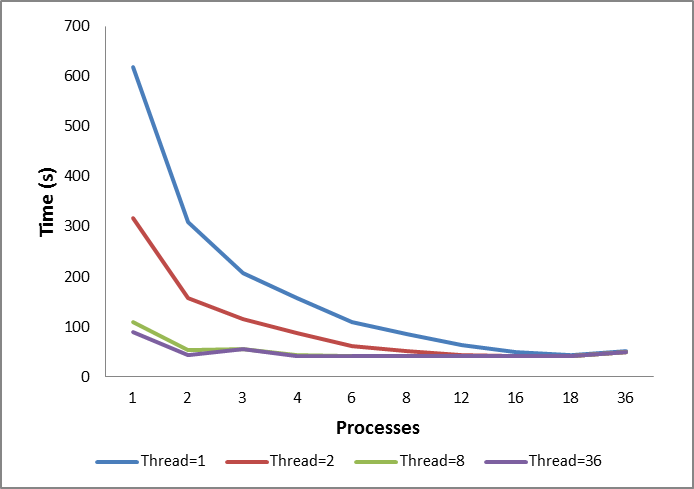
\includegraphics[width=.8\linewidth]{figures/threadComparison}
\caption{Comparison of elapsing time in hybrid model for fixed problem size $n = 16384$ and differing thread sizes $t \in\{1, 2, 8, 36\}$ }
\label{fig:hyb_th}
\end{figure}


\begin{table}
\centering
\begin{tabular}{c|c|c|c|c}
\hline
\multicolumn{5}{c}{$\tau$} \\
\hline \hline
    \backslashbox{\textbf{p}}{\textbf{t}} &1 &2 &8 &36\\ \hline
    
    % thread comp hybrid
1 &     6.174798de+02 &  3.171956de+02 &  1.097055de+02 &  8.927343de+01 \\
2 &     3.089000de+02 &  1.574979de+02 &  5.416437de+01 &  4.458945de+01 \\
3 &     2.073900de+02 &  1.148720de+02 &  5.646032de+01 &  5.604048de+01 \\
4 &     1.572596de+02 &  8.693238de+01 &  4.314681de+01 &  4.249215de+01 \\
6 &     1.102293de+02 &  6.204062de+01 &  4.178181de+01 &  4.144498de+01 \\
8 &     8.669200de+01 &  5.182738de+01 &  4.115636de+01 &  4.154543de+01 \\
12 &    6.365200de+01 &  4.310132de+01 &  4.092585de+01 &  4.148660de+01 \\
16 &    5.064756de+01 &  4.250397de+01 &  4.140603de+01 &  4.156513de+01 \\
18 &    4.476399de+01 &  4.183185de+01 &  4.186483de+01 &  4.164100de+01 \\
36 &    5.142002de+01 &  4.930061de+01 &  4.927885de+01 &  4.948230de+01 \\ 
\hline
\end{tabular}
\caption{Timing results of hybrid model with different threads for $n=16384$}
\label{table:hybrid_vs}
\end{table} 

\end{homeworkProblem}

\clearpage
\begin{homeworkProblem}{Speed-up and Parallel Efficiency}
The speed-up does not increase as much as the number of processes increases. The overhead of communication between processes does not allow the program perform much more efficiently. According to test results of the solver in Figure \ref{fig:speedEff} that was executed with different number of nodes, processes and threads, it comes out that the speed-up starts decreasing significantly for $36$ processes. This decrementing is due to communication overhead between large number of processes.\\
In the other hand, as the size of $n$ increases the speed-up increases which makes parallel programs useful for large problem sizes. But for small sizes like $n=64$ the speed-up $S_p$ is too low and the curve is decreasing. Graphs in Figure \ref{fig:speed_n} and \ref{fig:eff_n} are also illustrating how the communication overhead does affect the speedups. The parallel efficiency is decreased quickly when the processes have large values like $p=36$. So in order to make the program perform more efficiently, the number of processes must be scaled regarding the problem size. As the problem size increases, the achieved speed-ups also increase. But generally very large number of $P$ is not prefered because of unnecessary communication between processors. The situation in Figure \ref{fig:eff_n} is avoided by choosing a suitable value for $P$.\\

\begin{figure}[h]
% \centering
\begin{subfigure}{0.5\textwidth}
 \centering

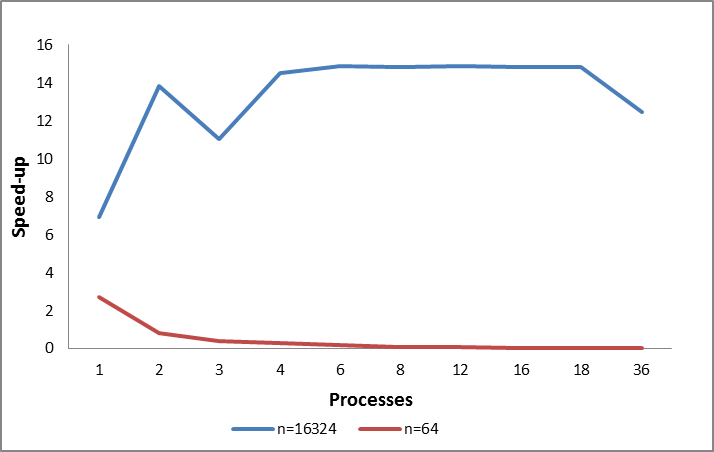
\includegraphics[width=\linewidth]{figures/2node_speedupNcomp}
\caption{Speed-ups}
\label{fig:speed_n}
\end{subfigure}
\begin{subfigure}{0.5\textwidth}
 \centering

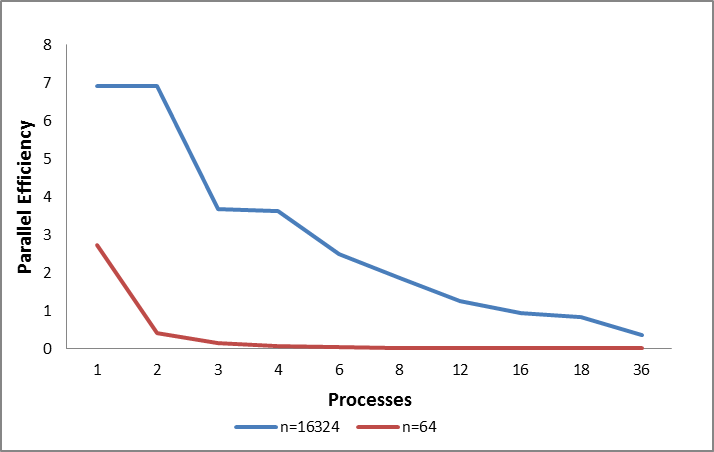
\includegraphics[width=\linewidth]{figures/2node_efficiencyNcomp}
\caption{Parallel Efficiency}
\label{fig:eff_n}
\end{subfigure}
\caption{Speedup and efficiency comparison when $n = 16384$ for different thread numbers. 2 cluster nodes. }
\label{fig:speedEff}
\end{figure}

\begin{table}
\centering
\begin{tabular}{c|c|c}
\hline
   \multicolumn{3}{c}{\textbf{Speedup $S_p$}}     \\ \hline \hline
\textbf{p}&   $n=16324$&    $n=64$ \\ \hline
1&  6.916726e+00&   2.735714e+00 \\
2&  1.384812e+01&   8.252589e-01 \\
3&  1.101846e+01&   4.053187e-01 \\
4&  1.453162e+01&   2.902934e-01 \\
6&  1.489879e+01&   1.536322e-01 \\
8&  1.486276e+01&   8.500874e-02 \\
12& 1.488384e+01&   5.077512e-02 \\
16& 1.485572e+01&   2.926936e-02 \\
18& 1.482865e+01&   2.493935e-02 \\
36& 1.247880e+01&   4.287743e-03 \\ \hline
\end{tabular}
\caption{Speedup comparison between small and big $n$ with $t=36$}
\end{table}

\begin{table}
\centering
\begin{tabular}{c|c|c}
\hline
   \multicolumn{3}{c}{\textbf{Parallel efficiency $\eta_p$}}     \\ \hline \hline
\textbf{p}&  $n=16324$&    $n=64$ \\ \hline
1&  6.916726e+00&   2.735714e+00 \\
2&  6.924058e+00&   4.126295e-01 \\
3&  3.672820e+00&   1.351062e-01 \\
4&  3.632905e+00&   7.257335e-02 \\
6&  2.483131e+00&   2.560536e-02 \\
8&  1.857845e+00&   1.062609e-02 \\
12& 1.240320e+00&   4.231260e-03 \\
16& 9.284823e-01&   1.829335e-03 \\
18& 8.238140e-01&   1.385519e-03 \\
36& 3.466334e-01&   1.191040e-04 \\ \hline
\end{tabular}
\caption{Parallel efficiency comparison between small and big $n$ with $t=36$}
\end{table}

\clearpage

Figure \ref{fig:th_cmp} illustrates a comparison of different thread sizes for fixed problem size  $n=2^{14}$. Similar behaviors compared to Figure \ref{fig:speedEff} is shown here too. 

\begin{figure}[h]
% \centering
\begin{subfigure}{0.5\textwidth}
 \centering
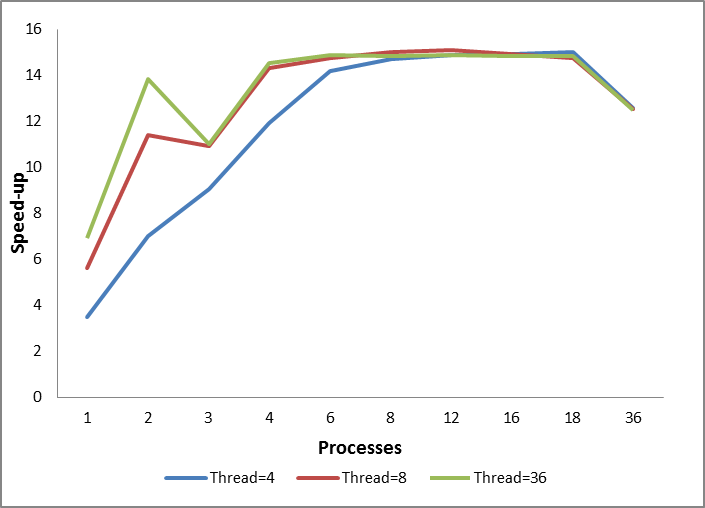
\includegraphics[width=\linewidth]{figures/2node_speedup_thComp16384}
\caption{Speed-ups}
\label{fig:speed_th}
\end{subfigure}
\begin{subfigure}{0.5\textwidth}
 \centering

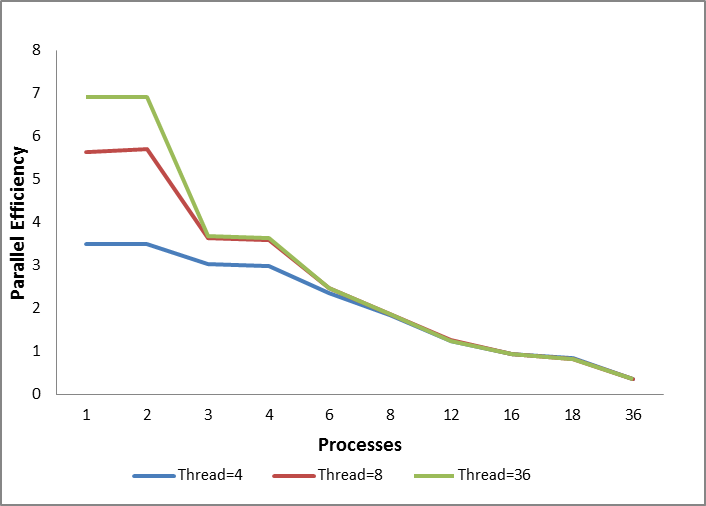
\includegraphics[width=\linewidth]{figures/2node_efficiency_thComp16384}
\caption{Parallel Efficiency}
\label{fig:eff_th}
\end{subfigure}
\caption{Speedup and efficiency comparison when $n = 16384$ for different thread numbers. 2 cluster nodes. }
\label{fig:th_cmp}
\end{figure}


\begin{table}[h!]
\centering
\begin{tabular}{c|c|c|c}
\hline
   \multicolumn{4}{c}{\textbf{Speedup $S_p$}}     \\ \hline \hline
\backslashbox{\textbf{p}}{\textbf{t}} & 4 & 8 & 36 \\ \hline
1&  3.492558e+00&   5.628521e+00&   6.916726e+00 \\
2&  7.007097e+00&   1.140011e+01&   1.384812e+01 \\
3&  9.058725e+00&   1.093653e+01&   1.101846e+01 \\
4&  1.192594e+01&   1.431114e+01&   1.453162e+01 \\
6&  1.419603e+01&   1.477868e+01&   1.489879e+01 \\
8&  1.471971e+01&   1.500327e+01&   1.486276e+01 \\
12& 1.489613e+01&   1.508777e+01&   1.488384e+01 \\
16& 1.492484e+01&   1.491280e+01&   1.485572e+01 \\
18& 1.503025e+01&   1.474937e+01&   1.482865e+01 \\
36& 1.256382e+01&   1.253032e+01&   1.247880e+01 \\ \hline
\end{tabular}
\caption{Speedup report for $n = 16384$.}
\end{table}

\begin{table}[h!]
\centering
\begin{tabular}{c|c|c|c}
\hline
   \multicolumn{4}{c}{\textbf{Parallel efficiency $\eta_p$}}     \\ \hline \hline
\backslashbox{\textbf{p}}{\textbf{t}} & 4 & 8 & 36 \\ \hline
1&  3.492558e+00&   5.628521e+00&   6.916726e+00 \\
2&  3.503549e+00&   5.700055e+00&   6.924058e+00 \\
3&  3.019575e+00&   3.645509e+00&   3.672820e+00 \\
4&  2.981485e+00&   3.577784e+00&   3.632905e+00 \\
6&  2.366005e+00&   2.463113e+00&   2.483131e+00 \\
8&  1.839964e+00&   1.875408e+00&   1.857845e+00 \\
12& 1.241344e+00&   1.257314e+00&   1.240320e+00 \\
16& 9.328022e-01&   9.320499e-01&   9.284823e-01 \\
18& 8.350138e-01&   8.194093e-01&   8.238140e-01 \\
36& 3.489950e-01&   3.480645e-01&   3.466334e-01 \\ \hline
\end{tabular}
\caption{Parallel efficiency report for $n = 16384$.}
\end{table}

\clearpage

\subsection{Performance Comparison for Different Node Size}
In order to see the performance differences between node sizes, the parallel program is executed on Lille for both 1 node and 2 nodes to see if there is any communication overhead when applying 2 nodes. A better performance is achieved when using 2 nodes.

\begin{figure}[h]
% \centering
\begin{subfigure}{0.5\textwidth}
 \centering

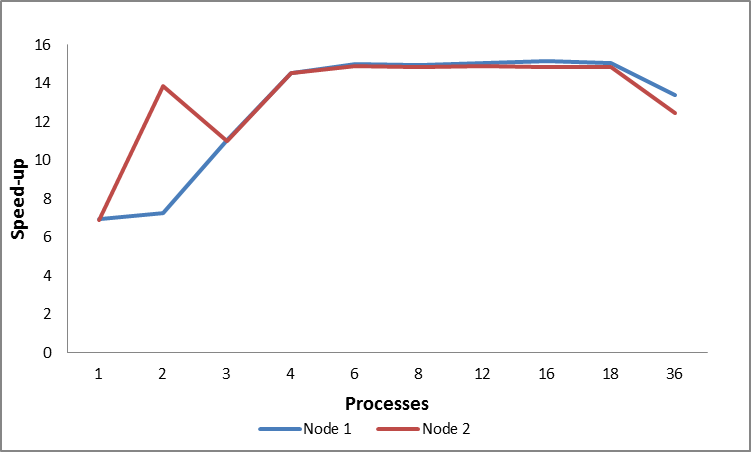
\includegraphics[width=\linewidth]{figures/4_Sp_node1_node2}
\caption{Speed-ups}
\label{fig:speed_th}
\end{subfigure}
\begin{subfigure}{0.5\textwidth}
 \centering

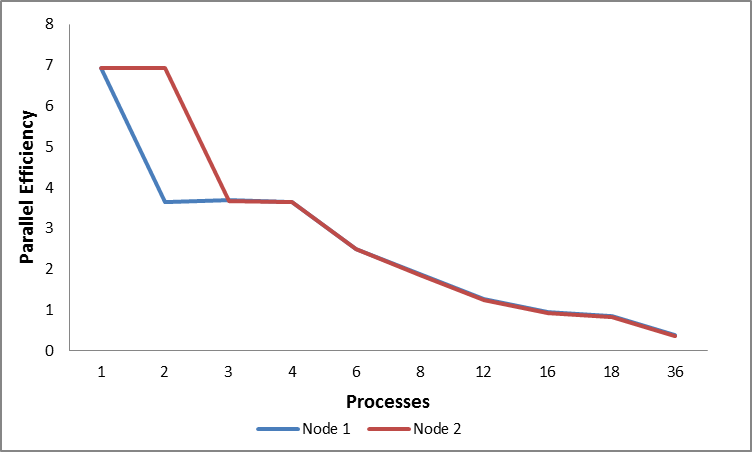
\includegraphics[width=\linewidth]{figures/4_eff_node1_node2}
\caption{Parallel Efficiency}
\label{fig:eff_th}
\end{subfigure}
\caption{Comparison of speedup and efficiency when $n = 16384$ for different numbers of cluster nodes. }
\end{figure}

\begin{table}[h!]
\centering
\begin{tabular}{l|c|c||c|c}
% \hline
%   \multicolumn{3}{c}{\textbf{Parallel efficiency $\eta_p$}}     \\ \hline
& \multicolumn{2}{c||}{\textbf{Parallel efficiency}} & \multicolumn{2}{c}{\textbf{Speedup}} \\ \hline
\backslashbox{\textbf{p}}{\textbf{node}}& 1 &    2 & 1 & 2 \\ \hline \hline
1&  6.930640e+00&   6.916726e+00 &  6.930640e+00&   6.916726e+00 \\
2&  3.627574e+00&   6.924058e+00 &  7.255147e+00&   1.384812e+01 \\
3&  3.686744e+00&   3.672820e+00 &  1.106023e+01&   1.101846e+01 \\
4&  3.629474e+00&   3.632905e+00 &  1.451790e+01&   1.453162e+01 \\
6&  2.498000e+00&   2.483131e+00 &  1.498800e+01&   1.489879e+01 \\
8&  1.871678e+00&   1.857845e+00 &  1.497342e+01&   1.486276e+01 \\
12& 1.255140e+00&   1.240320e+00 &  1.506168e+01&   1.488384e+01 \\
16& 9.482085e-01&   9.284823e-01 &  1.517134e+01&   1.485572e+01 \\
18& 8.371587e-01&   8.238140e-01 &  1.506886e+01&   1.482865e+01 \\
36& 3.714765e-01&   3.466334e-01 &  1.337315e+01&   1.247880e+01 \\
\end{tabular}
\caption{Parallel efficiency comparison for 1 and 2 cluster nodes.}
\end{table}

\begin{figure}[h]
% \centering
\begin{subfigure}{0.5\textwidth}
 \centering
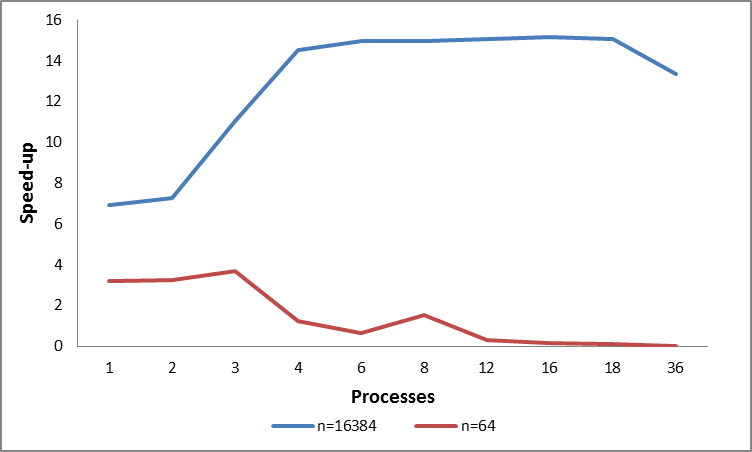
\includegraphics[width=\linewidth]{figures/4_Sp_node1_nComparison}
\caption{Speed-ups}
\label{fig:speed_th}
\end{subfigure}
\begin{subfigure}{0.5\textwidth}
 \centering

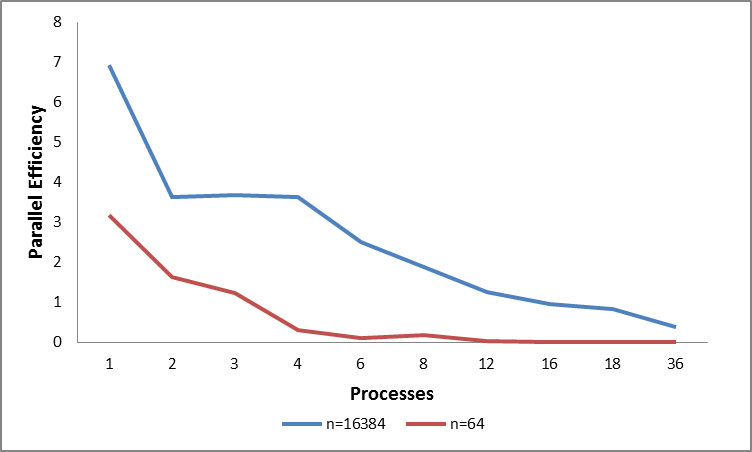
\includegraphics[width=\linewidth]{figures/4_eff_node1_nComparison}
\caption{Parallel Efficiency}
\label{fig:eff_th}
\end{subfigure}
\caption{Speedup and efficiency comparison when $n = 16384$ for different process numbers. 1 cluster nodes. }
\end{figure}

\end{homeworkProblem}

\clearpage
\begin{homeworkProblem}{Verification of Correctness}

Figure \ref{fig:error} shows the convergence for function $f$.

$$f(x,y) = -\Delta u= 5\pi ^2 sin(\pi x)sin(2 \pi y) $$ 

The convergence test confirms the correctness of parallel poisson solver implementation. The test results are as expected. In table \ref{table:conv} the maximum pointwise error is calculated for fixed number of processes in each test.

\begin{table}[h!]
\centering
\begin{tabular}{ l | l |l }
 \textbf{n} & \textbf{Time} & \textbf{Error} \\ \hline
16 &    1.212968e+00 &  3.208491e-01 \\
32 &    1.330465e+00 &  1.785441e-01 \\
64 &    1.351995e+00 &  9.374031e-02 \\
256 &   1.392981e+00 &  2.426724e-02 \\
512 &   1.329465e+00 &  1.220276e-02 \\
1024 &  3.045029e+00 &  6.118655e-03 \\
2048 &  3.907036e+00 &  3.063645e-03 \\
4096 &  7.759986e+00 &  1.532901e-03 \\
8192 &  2.534212e+01 &  7.667206e-04 \\
16384 & 9.371541e+01 &  3.834278e-04 \\
\end{tabular}
\caption{Convergence test shows the error which is decreased to zero as the problem size is increased.$P=18$, $t=8$}
\label{table:conv}
\end{table}

\begin{figure}[h!]
\centering
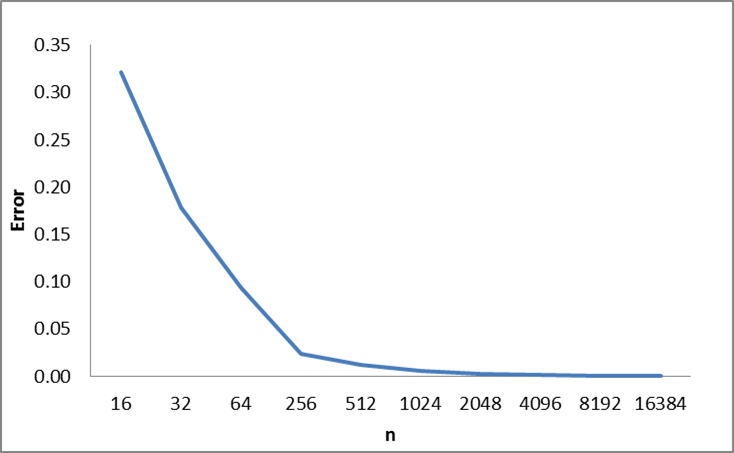
\includegraphics[width=.8\linewidth]{figures/convergence.png}
\caption{Convergence test showing decreasing of pointwise error when n increases}
\label{fig:error}
\end{figure}

\end{homeworkProblem}



\clearpage
\begin{homeworkProblem}{Disscussions}

The source code of Poisson solver must be modified in order to deal with different functions. If function $f(x,y)$ is changed, the only modification in the code should be on the \texttt{rhs(}\texttt{real} \texttt{x}, \texttt{real} \texttt{y)}. The convergence test for different $f$ must be implemented separately as well. 

\subsubsection{Efficiency Improvement}
The transpose operation is the part of implementation that slows down the program. It requires a lot of communication between processes. In addition, there are two nested loops in the \texttt{prallal\_transpose} function. The performance could be more efficient if this function operates faster. Dynamic programming could be tried in order to boost the transpose algorithm. 
\subsubsection{Non-homogeneous Dirichlet Boundary Conditions}
According to the course's lecture notes, the solution for non-homogeneous Dirichlet boundary can be used in order to solve it for this problem. To include the boundary points  we have to add a new vector $b$ to the right hand side of the equation to express the system as $Au = g$ and so the left hand side will be exactly the same. So the new equation will be defined as $G =  h^2 f + b$.
\[
\textbf{G}=h^2
  \begin{bmatrix}
    f_{1,1}   & \hdots & f_{1,n-1} \\
    \vdots & \ddots & \vdots \\
    f_{n-1,1} & \hdots & f_{n-1,n-1}
  \end{bmatrix}
  +
   \begin{bmatrix}
    u_{0,0}   & \hdots & u_{0,n} \\
    \vdots & \text{0} & \vdots \\
    u_{n,0} & \hdots & u_{n,n}
  \end{bmatrix}
\]
The Poisson solver represented in this report assumes that $u=0$. The program assumption is that every other point out of the given boundary is equal zero .
In order to support non-homogeneous Dirchlet boundary conditions where $u\ne0$, the boundaries should be specified and stored. So the points out of its domain must be checked in order to find non-zero points. This checking operation could be done within the right hand side function. Modifications in \texttt{rhs} function could improve the program to deal with non-homogeneous Dirchlet Boundary conditions.
\subsubsection{Rectangular Matrices}
The parallel solver allows only square matrices. The source code could be improved in a way that it operates on rectangular matrices too. The length in both x-direction and y-direction in this project is defined as $L=1$. Consequently $h = \frac{1}{n}$.
One improvement could be assuming distinct step size in each direction. By defining $h_x$ and $h_y$ the problem is easily solved.
$$ h_x = \frac{L_x}{n} $$
$$ h_y = \frac{L_y}{n} $$
So the domain would be as following,

$$ \Omega = (0, L_x) \times (0, L_y) $$.\\


\end{homeworkProblem}

\begin{homeworkProblem}{Appendix}

\subsection{Environment and Compiler Information}

Modules:\\
openmpi/2.0.1\\
gcc/6.3.0\\

cmake version 2.8.12.2\\~\\

Kernel name : linux\\
Nodename :  lille\-login1.foreman.hpc.ntnu.no\\
Kernel release: 3.10.0\-514.10.2.el7.x86\_64\\
Kernel version: \#1 SMP Fri Mar 3 00:04:05 UTC 2017\\
Machine hardware: x86\_64\\
Processor type: x86\_64\\
hardware platform: x86\_64\\
Operating system : GNU/Linux \\

\subsection{System Architecture}

\end{homeworkProblem}

\begin{homeworkProblem}{References}
http://thebb.github.io/TMA4280/notes.pdf \\

\end{homeworkProblem}
%----------------------------------------------------------------------------------------

\end{document}
